\begin{center}	
\textbf{BOLETÍN DE EJERCICIOS 2}
\end{center}

\vspace{.2cm}

\begin{enumerate}[\bfseries \mbox{EJERCICIO} 1.]

    %-------------------- EJERCICIO 1
    \item Reproduzca para España y el país elegido por su grupo el siguiente cuadro del mercado laboral con los últimos datos disponibles.\\\\

	\begin{tcolorbox}[colframe=white!30!black, title=La Actividad laboral en España  en millones de personas (EPA 2023:1)]
	\begin{center}
	    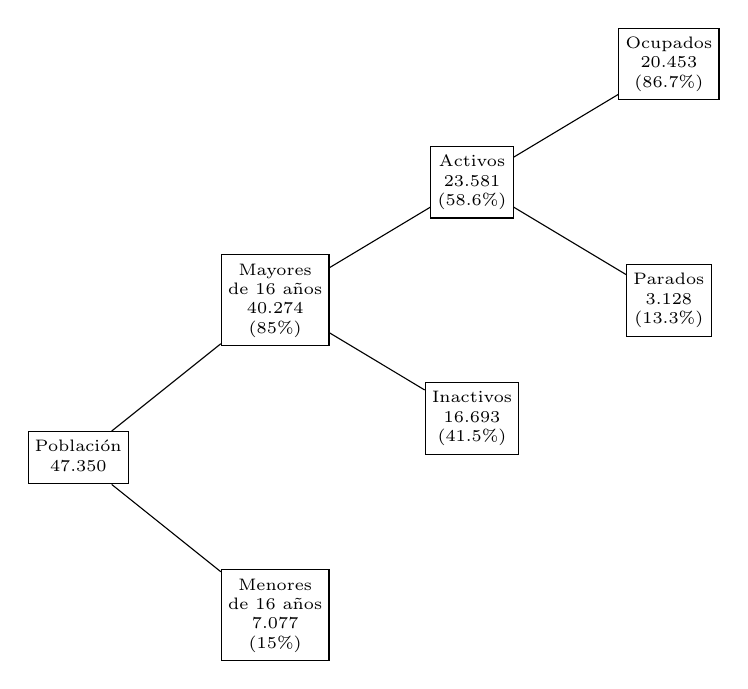
\begin{tikzpicture}[scale=1,level distance=2.5cm,
				level 1/.style={sibling distance=4cm},
				level 2/.style={sibling distance=3cm},
				every node/.style={draw},
				grow'=right]
	      % Definir los nodos del árbol
	      {\fontsize{6}{7}\selectfont
	      \node {%
		  \begin{tabular}{@{}c@{}}
		      Población\\
		      47.350
		   \end{tabular}
	      }
		child {node {%
		  \begin{tabular}{@{}c@{}}
		      Mayores\\ de 16 años\\
		      40.274\\
		      (85\%)
		   \end{tabular}
		    }
		  child {node {%
		  \begin{tabular}{@{}c@{}}
		      Activos\\
		      23.581\\
		      (58.6\%)
		   \end{tabular}
		      }
		      child {node {%
		      \begin{tabular}{@{}c@{}}
			  Ocupados\\
			  20.453\\
			  (86.7\%)
		       \end{tabular}
		      }}
		      child {node {%
		      \begin{tabular}{@{}c@{}}
			  Parados\\
			  3.128\\
			  (13.3\%)
		       \end{tabular}
		      }}
		  }
		  child {node {%
		  \begin{tabular}{@{}c@{}}
		      Inactivos\\
		      16.693\\
		      (41.5\%)
		   \end{tabular}
		  }}
		}
		child {node {%
		  \begin{tabular}{@{}c@{}}
		      Menores\\ de 16 años\\
		      7.077\\
		      (15\%)
		   \end{tabular}
		    }
		};
	    }
	    \end{tikzpicture}
	\end{center}
    \end{tcolorbox}

    \vspace{.5cm}

	\begin{tcolorbox}[colframe=white!30!black, title=La Actividad laboral en Alemania  en millones de personas (Destatis 2021:12)]
	\begin{center}
	    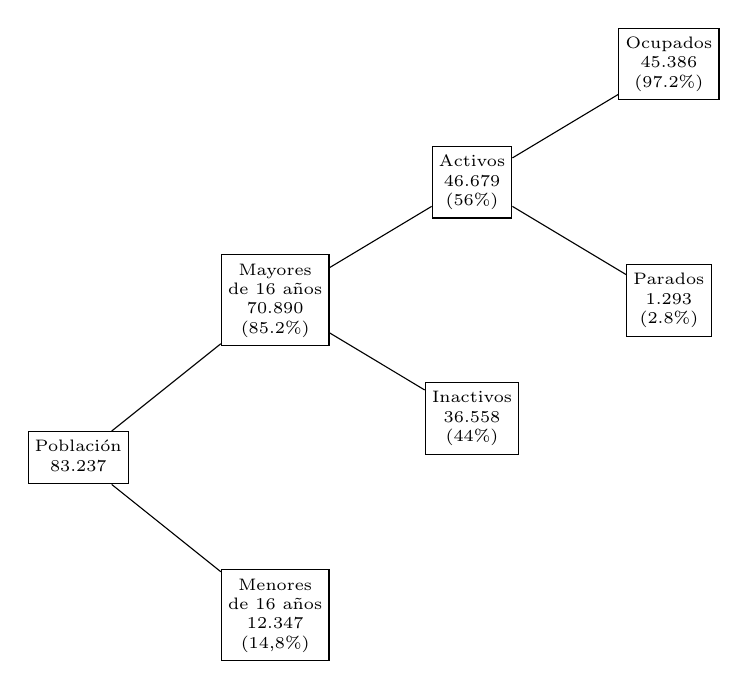
\begin{tikzpicture}[scale=1,level distance=2.5cm,
				level 1/.style={sibling distance=4cm},
				level 2/.style={sibling distance=3cm},
				every node/.style={draw},
				grow'=right]
	      % Definir los nodos del árbol
	      {\fontsize{6}{7}\selectfont
	      \node {%
		  \begin{tabular}{@{}c@{}}
		      Población\\
		      83.237
		   \end{tabular}
	      }
		child {node {%
		  \begin{tabular}{@{}c@{}}
		      Mayores\\ de 16 años\\
		      70.890\\
		      (85.2\%)
		   \end{tabular}
		    }
		  child {node {%
		  \begin{tabular}{@{}c@{}}
		      Activos\\
		      46.679\\
		      (56\%)
		   \end{tabular}
		      }
		      child {node {%
		      \begin{tabular}{@{}c@{}}
			  Ocupados\\
			  45.386\\
			  (97.2\%)
		       \end{tabular}
		      }}
		      child {node {%
		      \begin{tabular}{@{}c@{}}
			  Parados\\
			  1.293\\
			  (2.8\%)
		       \end{tabular}
		      }}
		  }
		  child {node {%
		  \begin{tabular}{@{}c@{}}
		      Inactivos\\
		      36.558\\
		      (44\%)
		   \end{tabular}
		  }}
		}
		child {node {%
		  \begin{tabular}{@{}c@{}}
		      Menores\\ de 16 años\\
		      12.347\\
		      (14,8\%)
		   \end{tabular}
		    }
		};
	    }
	    \end{tikzpicture}
	\end{center}
    \end{tcolorbox}

    \vspace{.5cm}

    %-------------------- EJERCICIO 2	
    \item Actualice para el ultimo trimestre disponible, para España y el País elegido el siguiente cuadro.

    \begin{table}[htbp]
      \centering
      \caption{CIFRAS DEL MERCADO DE TRABAJO ESPAÑA (I)}
      \begin{center}
	  Primer trimestre de 2023
      \end{center}
      \scalebox{0.48}{
	\begin{tabular}{l|c|c|c}
	\toprule
	     \multicolumn{1}{l}{} & \multicolumn{1}{l}{Total} & \multicolumn{1}{l}{Varones} & \multicolumn{1}{l}{Mujeres}\\
	\midrule
	     \begin{tabular}{@{}l@{}}Tasa de actividad\\(activos en \% de población en edad de trabajar)\end{tabular}&58,55&63,18&54,18\\
	     \begin{tabular}{@{}l@{}}Tasa de empleo\\(empleados en \% de población en edad de trabajar)\end{tabular}&50,78&55,87&45,99\\
											Tasa de paro&&&\\
												    \quad 16-19 años&46,91&47,63&46,05\\
												    \quad 20-24 años&26,73&25,27&28,42\\
												    \quad 25-54 años&12,13&10,26&14,16\\
												    \quad 55 y más años&11,79&10,35&13,44\\
	\bottomrule
	\end{tabular}%
	}
      \label{tab:addlabel}%
      \begin{center}
      \tiny Fuente: INE.es.
      \end{center}
    \end{table}
    \vspace{.5cm}

    \begin{table}[htbp]
      \centering
      \caption{CIFRAS DEL MERCADO DE TRABAJO ALEMANIA (I)}
      \begin{center}
	  Cuarto trimestre del 2022
      \end{center}
      \scalebox{0.48}{
	\begin{tabular}{l|c|c|c}
	\toprule
	     \multicolumn{1}{l}{} & \multicolumn{1}{l}{Total} & \multicolumn{1}{l}{Varones} & \multicolumn{1}{l}{Mujeres}\\
	\midrule
	     \begin{tabular}{@{}l@{}}Tasa de actividad\\(activos en \% de población en edad de trabajar)\end{tabular}&70,2&74,6&65,7\\
	     \begin{tabular}{@{}l@{}}Tasa de empleo\\(empleados en \% de población en edad de trabajar)\end{tabular}&68,1&72,3&63,9\\
											Tasa de paro&&&\\
												    \quad 15-25 años&4.5&5.5&5.5\\
												    \quad 25-75 años&2.7&2.8&2.6\\
	\bottomrule
	\end{tabular}%
	}
      \label{tab:addlabel}%
      \begin{center}
      \tiny Fuente: Eurostat, Destatis.
      \end{center}
    \end{table}
    \vspace{.5cm}


    %-------------------- EJERCICIO 3
    \item Actualice para el ultimo trimestre disponible, el siguiente cuadro.

    \begin{table}[htbp]
      \centering
      \caption{CIFRAS DEL MERCADO DE TRABAJO, ESPAÑA (II)}
      \begin{center}
	  Primer trimestre de 2023 (\%)
      \end{center}
      \scalebox{0.483}{
	\begin{tabular}{l|r}
	\toprule
	     \multicolumn{1}{l}{Comunidades} & \multicolumn{1}{c}{Total}\\
	\midrule
	     Tasa de paro: nacional &13.26\\
	    \quad Andalucía&18,31\\
	    \quad Aragón&8,94\\
	    \quad Principado de Asturias&13,06\\
	    \quad Illes Balears&18,14\\
	    \quad Canarias&17,17\\
	    \quad Cantabria&9,29\\
	    \quad Castilla y León&10,28\\
	    \quad Castilla - La Mancha&15,02\\
	    \quad Cataluña&10,37\\
	    \quad Comunitat Valenciana&13,78\\
	    \quad Extremadura&19,53\\
	    \quad Galicia&10,90\\
	    \quad Comunidad de Madrid&11,01\\
	    \quad Región de Murcia&13,48\\
	    \quad Comunidad Foral de Navarra&12,13\\
	    \quad País Vasco&8,44\\
	    \quad La Rioja&10,06\\
	    \quad Ceuta&23,97\\
	    \quad Melilla&26,06\\
	\bottomrule
	\end{tabular}%
	}
      \label{tab:addlabel}%
      \begin{center}
      \tiny Fuente: INE.es.
      \end{center}
    \end{table}
    \vspace{.5cm}


    \begin{table}[htbp]
      \centering
      \caption{CIFRAS DEL MERCADO DE TRABAJO DE ALEMANIA (II)}
      \begin{center}
	  A febrero de 2023 (\%)
      \end{center}
      \scalebox{0.5}{
	\begin{tabular}{l|r}
	\toprule
	     \multicolumn{1}{l}{Comunidades} & \multicolumn{1}{c}{Total}\\
	\midrule
	     Tasa de paro: nacional &2.9\\
	     \quad Baden-Wurtemberg & 3.8\\
	     \quad Bayern & 3.6\\
	     \quad Berlin & 9.1\\
	     \quad Brandenburg & 6.7\\
	     \quad Bremen & 10.5\\
	     \quad Hamburg & 8.1\\
	     \quad Hessen & 5.2\\
	     \quad Mecklenburg-Vorpommern & 8.4\\
	     \quad Niedersachsen & 6.2\\
	     \quad Nordrhein-Westfalen & 7.8\\
	     \quad Rheinland-Pfalz & 4.9\\
	     \quad Saarland & 6.8\\
	     \quad Sachsen & 6.2\\
	     \quad Sachsen-Anhalt & 7.8\\
	     \quad Schleswig-Holstein & 6.2\\
	     \quad Thüringen & 6.1\\
	\bottomrule
	\end{tabular}%
	}
      \label{tab:addlabel}%
      \begin{center}
      \tiny Fuente: Celcdata.
      \end{center}
    \end{table}
    \vspace{1cm}



    %-------------------- EJERCICIO 4
    \item Actualice para el ultimo trimestre disponible, para España y los países de la UE 28 el siguiente cuadro.\\\\


    \begin{table}[htbp]
      \centering
      \caption{CIFRAS DEL MERCADO DE TRABAJO (III)}
      \begin{center}
	  Primer trimestre de 2023 (\% del empleo total)\\
	  \scriptsize De 15 a 74 años
      \end{center}
      \scalebox{.5}{
	\begin{tabular}{lr}
	\toprule
	     \multicolumn{1}{l}{} & \multicolumn{1}{c}{Total}\\
	\midrule
	    Asalariados a tiempo completo&86.5\\
	    Asalariados a tiempo parcial&13,5\\
	    \quad Bélgica&24,2\\
	   \quad Bulgaria&1,9\\
	   \quad Republica Checa&7,1\\
	   \quad Dinamarca&26,1\\
	   \quad Alemania&29,6\\
	   \quad Estonia&15,6\\
	   \quad Irlanda&21,3\\
	   \quad Grecia&8,0\\
	   \quad Francia&17,1\\
	   \quad Croacia&5,7\\
	   \quad Italia&17,8\\
	   \quad Chipre&9,8\\
	   \quad Letonia&7,6\\
	   \quad Lituania&7,1\\
	   \quad Luxemburgo&18,3\\
	   \quad Hungría&5,1\\
	   \quad Malta&12,3\\
	   \quad Países Bajos&43,2\\
	   \quad Austria&30,6\\
	   \quad Polonia&6,2\\
	   \quad Portugal&7,6\\
	   \quad Rumania&3,7\\
	   \quad Eslovenia&8,5\\
	   \quad Eslovaquia&3,4\\
	   \quad Finlandia&18,6\\
	   \quad Suecia&22,0\\
	   \quad Islandia&22,6\\
	   \quad Noruega&25,7\\
	   \quad Zuiza&39,3\\
	   \quad Serbia&6,6\\
	   \quad European Union&18,4\\
	   Asalariados contrato indefinido&84.9\\
	   Asalariados contrato temporal&14,9\\
	\bottomrule
	\end{tabular}%
	}
      \label{tab:addlabel}%
      \begin{center}
      \tiny Fuente: Eurostat.
      \end{center}
    \end{table}
    \vspace{2.5cm}


    %-------------------- EJERCICIO 5
    \item Actualice para el ultimo trimestre disponible, para España y el País elegido el siguiente cuadro:\\\\


	\begin{center}
	    \includegraphics[scale=0.27]{image/tasa_crecimiento.png}
	\end{center}

	\begin{center}
	    \includegraphics[scale=0.27]{image/tasa_crecimientoA.png}
	\end{center}

\newpage

    %-------------------- EJERCICIO 6
    \item Actualice para el ultimo trimestre disponible, para España y el País elegido el siguiente cuadro.

	\begin{center}
	    \includegraphics[scale=0.27]{image/tasa_desempleo.png}
	\end{center}
	\begin{center}
	    \includegraphics[scale=0.27]{image/tasa_desempleoA.png}
	\end{center}
	\vspace{.5cm}

\newpage

    %-------------------- EJERCICIO 7
    \item  Actualice para el ultimo trimestre disponible, para España y el País elegido el siguiente cuadro:

	\begin{center}
	    \includegraphics[scale=0.26]{image/porcentaje_asalariados_completo.png}
	\end{center}
	\vspace{.5cm}

	\begin{center}
	    \includegraphics[scale=0.26]{image/porcentaje_asalariados_indefinido.png}
	\end{center}
	\vspace{.5cm}

	\begin{center}
	    \includegraphics[scale=0.26]{image/porcentaje_parados_masdeunaño.png}
	\end{center}
	\vspace{.5cm}

	\begin{table}[htbp]
      \centering
      \caption{EMPLEO Y DESEMPLEO EN ESPAÑA}
      \begin{center}
	\tiny Comparación de Fuentes
      \end{center}
      \scalebox{0.5}{
      \begin{tabular}{l*{4}{r}l*{3}{r}}
	\toprule
	& \multicolumn{4}{c}{Miles de personas} & \multicolumn{3}{c}{(\%) crec. anual} \\
	\cmidrule(lr){2-5} \cmidrule(lr){6-8}
	& 2019 & 2020 & 2021 & 2022 & 2020 & 2021 & 2022 \\
	\midrule
	\textbf{EPA} 		   		&&&&&&& \\
	Ocupados 			  	&19.779&19.202&19.774&20.391&-2.9&2.9&3.1\\\\
	\textbf{Seguridad social} 		&&&&&&& \\
	Efectivos 				&19.408&19.048&19.825&20.296&-1.9&4.1&2.4\\\\
	\textbf{Contabilidad Nacional} 		&&&&&&& \\
	Empleados equivalentes 			&&&&&&& \\
	\qquad a tiempo completo 		&18.490&17.225&18.362&&-6.8&6.6& \\
	Empleo total				&21.026&18.793&18.998&&-10.6&1.1& \\\\
	\textbf{EPA} 				&&&&&&& \\
	Parados 				&3.247&3.531&3.429&3.025&8.7&-2.9&-11.8\\\\
	\textbf{INEM} 				&&&&&&& \\
	Parados 				&3.163&3.888&3.106&2.897&22.9&-20.1&-6.7\\
	Beneficiarios prestaciones 		&&&&&&& \\
	\bottomrule
      \end{tabular}%
      }
      \label{tab:addlabel}%
    \end{table}
    \vspace{1cm}


    %-------------------- EJERCICIO 8
    \item Actualice para el último trimestre disponible, los siguientes cuadros:\\\\

    \begin{table}[htbp]
      \centering
      \caption{TASA DE EMPLEO}
      \begin{center}
	  Cuarto trimestre del 2022 (15 años o más)\\
      \end{center}
      \scalebox{0.5}{
	\begin{tabular}{lr}
	\toprule
	     \multicolumn{1}{l}{\quad Países} & \multicolumn{1}{c}{\%}\\
	\midrule
	   \quad Bélgica&66,8\\
	   \quad Bulgaria&71,5\\
	   \quad Republica Checa&75.8\\
	   \quad Dinamarca&76,9\\
	   \quad Alemania&77,3\\
	   \quad Estonia&76,9\\
	   \quad Irlanda&73,2\\
	   \quad Grecia&60,7\\
	   \quad España&64,3\\
	   \quad Francia&68,2\\
	   \quad Croacia&65,6\\
	   \quad Italia&60,7\\
	   \quad Chipre&73,1\\
	   \quad Letonia&71,3\\
	   \quad Lituania&72,8\\
	   \quad Luxemburgo&69,6\\
	   \quad Hungría&74,5\\
	   \quad Malta&78,5\\
	   \quad Países Bajos&82,2\\
	   \quad Austria&74.0\\
	   \quad Polonia&71,8\\
	   \quad Portugal&71,6\\
	   \quad Rumania&62,8\\
	   \quad Eslovenia&73.0\\
	   \quad Eslovaquia&71,8\\
	   \quad Finlandia&74,3\\
	   \quad Suecia&76,8\\
	   \quad Islandia&83,3\\
	   \quad Noruega&77,3\\
	   \quad Zuiza&79,9\\
	   \quad Serbia&64,2\\
	   \quad European Union&70,1\\
	\bottomrule
	\end{tabular}%
	}
      \label{tab:addlabel}%
      \begin{center}
      \tiny Fuente: Eurostat.
      \end{center}
    \end{table}


    \begin{table}[htbp]
      \centering
      \caption{TASA DE EMPLEO}
      \begin{center}
	  Cuarto trimestre del 2022 (de 55 a 64 años)\\
      \end{center}
      \scalebox{0.5}{
	\begin{tabular}{lr}
	\toprule
	     \multicolumn{1}{l}{\quad Países} & \multicolumn{1}{c}{\%}\\
	\midrule
	   \quad Bélgica&57,5\\
	   \quad Bulgaria&59,4\\
	   \quad Republica Checa&73,1\\
	   \quad Dinamarca&73,1\\
	   \quad Alemania&73,8\\
	   \quad Estonia&75,3\\
	   \quad Irlanda&67,3\\
	   \quad Grecia&52,8\\
	   \quad España&58,0\\
	   \quad Francia&57,2\\
	   \quad Croacia&51,4\\
	   \quad Italia&56,0\\
	   \quad Chipre&65,3\\
	   \quad Letonia&70,3\\
	   \quad Lituania&69,5\\
	   \quad Luxemburgo&44,4\\
	   \quad Hungría&66,8\\
	   \quad Malta&56,3\\
	   \quad Países Bajos&73,9\\
	   \quad Austria&56,7\\
	   \quad Polonia&57,3\\
	   \quad Portugal&66,2\\
	   \quad Rumania&47,1\\
	   \quad Eslovenia&55,2\\
	   \quad Eslovaquia&65,6\\
	   \quad Finlandia&72,2\\
	   \quad Suecia&77,9\\
	   \quad Islandia&82,5\\
	   \quad Noruega&73,9\\
	   \quad Zuiza&72,5\\
	   \quad Serbia&53,9\\
	   \quad European Union&62.9\\
	\bottomrule
	\end{tabular}%
	}
      \label{tab:addlabel}%
      \begin{center}
      \tiny Fuente: Eurostat.
      \end{center}
    \end{table}

    \begin{center}
	\includegraphics[width=0.8\textwidth]{image/porcentaje_emeplo_union_europea.png}
    \end{center}

    \begin{table}[htbp]
      \centering
      \caption{TASA DE PARO}
      \begin{center}
	  Cuarto trimestre del 2022 (de 15 a 74 años)\\
      \end{center}
      \scalebox{0.5}{
	\begin{tabular}{lr}
	\toprule
	     \multicolumn{1}{l}{\quad Países} & \multicolumn{1}{c}{\%}\\
	\midrule
	   \quad Bélgica&6,1\\
	   \quad Bulgaria&5,7\\
	   \quad Republica Checa&3,9\\
	   \quad Dinamarca&4,7\\
	   \quad Alemania&3,1\\
	   \quad Estonia&5,4\\
	   \quad Irlanda&4,4\\
	   \quad Grecia&11,8\\
	   \quad España&12,9\\
	   \quad Francia&7,2\\
	   \quad Croacia&6,6\\
	   \quad Italia&7,9\\
	   \quad Chipre&7,1\\
	   \quad Letonia&6,8\\
	   \quad Lituania&6,1\\
	   \quad Luxemburgo&4,6\\
	   \quad Hungría&3,9\\
	   \quad Malta&2,9\\
	   \quad Países Bajos&3,5\\
	   \quad Austria&5,0\\
	   \quad Polonia&2,9\\
	   \quad Portugal&6,5\\
	   \quad Rumania&5,6\\
	   \quad Eslovenia&3,6\\
	   \quad Eslovaquia&6,0\\
	   \quad Finlandia&6,8\\
	   \quad Suecia&7,4\\
	   \quad Islandia&3,5\\
	   \quad Noruega&3,3\\
	   \quad Zuiza&4,4\\
	   \quad Serbia&9,3\\
	   \quad European Union&6,1\\
	\bottomrule
	\end{tabular}%
	}
      \label{tab:addlabel}%
      \begin{center}
      \tiny Fuente: Eurostat.
      \end{center}
    \end{table}


\end{enumerate}
